% This is samplepaper.tex, a sample chapter demonstrating the
% LLNCS macro package for Springer Computer Science proceedings;
% Version 2.20 of 2017/10/04
%
\documentclass[runningheads]{llncs}
%
\usepackage{graphicx}
\usepackage{float}
% Used for displaying a sample figure. If possible, figure files should
% be included in EPS format.
%
% If you use the hyperref package, please uncomment the following line
% to display URLs in blue roman font according to Springer's eBook style:
% \renewcommand\UrlFont{\color{blue}\rmfamily}
\graphicspath{ {images/} }

\begin{document}
%
\title{\textbf{Java Path Finder}
}
%
%\titlerunning{Abbreviated paper title}
% If the paper title is too long for the running head, you can set
% an abbreviated paper title here%

\author{Farias Juan\inst{1}\and
Kokic Emiliano\inst{1} \and
Moresi Marco\inst{1}}
%
\authorrunning{Farias Juan, Kokic Emiliano, Moresi Marco}
% First names are abbreviated in the running head.
% If there are more than two authors, 'et al.' is used.
%
\institute{Facultad de Matem\'atica, Astronom\'ia, F\'isica y Computaci\'on, C\'ordoba, Argentina
\email{\{frsjuanignacio, emikokic, mrc.moresi\}@gmail.com}}
%

\maketitle              % typeset the header of the contribution
%
\begin{abstract}
Esta investigaci\'on se centr\'o en el funcionamiento de la herramienta Java Path Finder, la cual permite verificar programas escritos en Java. Se investig\'o sobre distintos aspectos t\'ecnicos de la misma como as\'i tambi\'en aspectos de usabilidad e interacci\'on con el usuario.
Dado lo vers\'atil de la herramienta, decidimos acotar la investigaci\'on s\'olo al uso de JPF como model checker de programas concurrentes. Esta investigaci\'on aporta un an\'alisis para aquellos nuevos usuarios de esta herramienta originalmente desarrollada por la NASA y actualmente de c\'odigo abierto.


\keywords{JPF \and Model Checker \and Java.}
\end{abstract}
%
%
%
\section{Contexto de creaci\'on de la herramienta}

Java Path Finder, tambi\'en como conocido como JPF,  se comenz\'o a desarrollar en el a\~no  1999 como un traductor de Java a Promela[1] (usando Spin[2] como model checker). Para el a\~no 2000, se convirti\'o en una herramienta de model checker por si sola, dejando de lado la utilizaci\'on de Spin. Las primeras etapas fueron desarrolladas por el grupo Robust Software Engineering en la NASA Ames Research Center, junto con el apoyo de organizaciones tales como RIACS (The Research Institute for Advanced Computer Science).
En el a\~no 2005 se convirti\'o en una herramienta de c\'odigo abierto. Actualmente, se encuentra disponible de manera gratuita y en desarrollo continuo gracias al apoyo de m\'as de 20 universidades de todo el mundo.

\begin{figure}
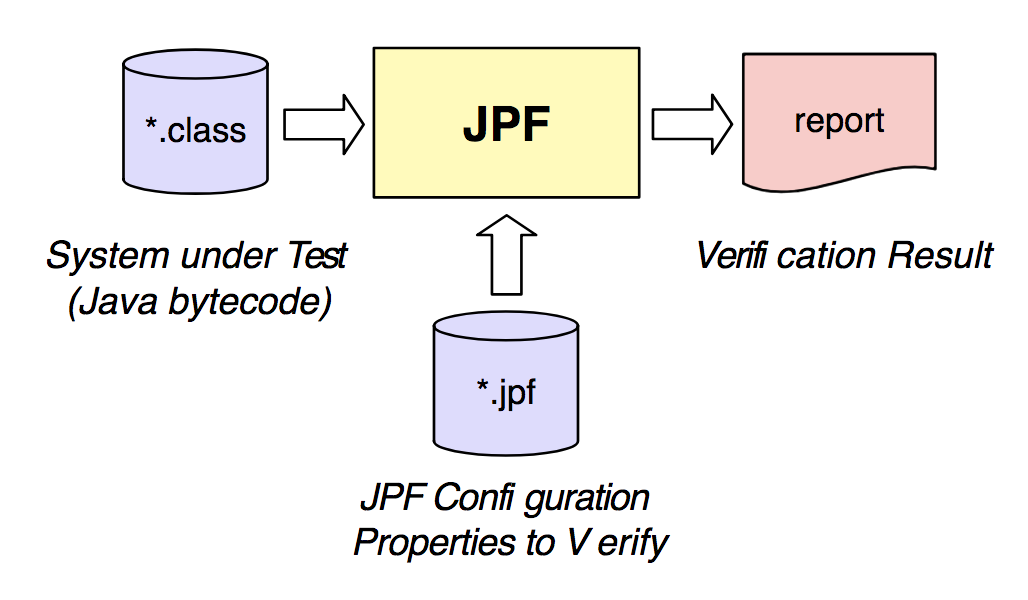
\includegraphics[width=\textwidth]{fig1.png}
\caption{The Core : a VM that supports Model Checking} \label{fig1}
\end{figure}

\section{Objetivo de la herramienta}



El objetivo de JPF depende como se configure la herramienta, el n\'ucleo principal de JPF es una Java Virtual Machine que ejecuta c\'odigo compilado de Java (Java Bytecode)(ver Figura 1). Es utilizado para detectar defectos, para lo cual, JPF toma como entrada el programa a verificar y la configuraci\'on que se desea verificar (archivo .jpf). JPF devolver\'a un reporte describiendo si las propiedades de la configuraci\'on se mantienen y/o que artefactos de verificaci\'on han sido creados por JPF para su posterior an\'alisis. 
Un an\'alisis realizado por JPF por defecto (es decir, sin agregarle una configuraci\'on personalizada por el usuario) hace uso de una caracter\'istica importante de JPF: execution choices. JPF puede identificar puntos en el programa donde la ejecuci\'on puede proceder de diferentes maneras, luego explora sistem\'aticamente cada uno de estos puntos, es decir, JPF ejecuta todos los caminos posibles. En cuanto al n\'umero de caminos, puede crecer exponencialmente (esto es llamado como \textit{state explosion problem}). Para lidiar con esto, JPF emplea una linea de defensa llamada chequeo de estados: cada vez que JPF alcanza un punto de elecci\'on, checkea si ya ha visto un estado similar en el programa y en tal caso, abandona ese camino, realiza un vuelta atr\'as a un punto de elecci\'on previo que tenga posibles elecciones no exploradas y procede desde alli. 
En caso de ejecutar sin una configuraci\'on propia, por defecto JPF verificar\'a el programa en b\'usqueda de deadlocks y excepciones no controladas (unhandled exceptions). Estas son llamadas propiedades non-funcional. Pero como se mencion\'o previamente, el usuario puede definir propiedades espec\'ificas, que en su mayor\'ia, se realizan con los llamados listeners (peque\~nos ‘plugins’ que permiten monitorear con mas detalle todas las acciones que va tomando JPF). Todo explica porque JPF es llamado "a debugger toolbox on steroids", primero autom\'aticamente ejecuta el programa de entrada en todas sus formas posibles para detectar defectos y cuando los encuentra muestra una explicaci\'on de que lo caus\'o. Y luego puede ser extendido en base a la necesidad del usuario.


\section{Descripci\'on de la herramienta del lado del usuario}

JPF no presenta interfaz gr\'afica propia, pero permite ser ejecutado de diversas maneras. Se puede utilizar desde la linea de comandos, como asi tambi\'en desde los diversos IDE de desarrollo para Java como NetBeans o Eclipse donde es necesario instalar los plugins correspondientes. M\'as a\'un se puede integrar JPF a un programa de Java como una clase embebida.
Adem\'as se puede ejecutar desde JUnit el framework de java para escribir Unit Test.


\section{Aspectos t\'ecnicos de la herramienta}

JPF fue dise\~nanda en base a dos abstracciones, la VM (m\'aquina virtual), y Search Component.
La encargada de generar los estados es la VM, mediante la ejecuci\'on de instrucciones en Java Byte Code, la VM  genera la representaci\'on de los estados, los cuales pueden ser:

\begin{itemize}
\item Verificados por igualdad (es decir, si el estado ha sido visitado antes).
\item Analizados (ver los valores que contiene).
\item Almacenados.
\item Restaurados.
\end{itemize}

Search Component[9] es el responsable de elegir el siguiente estado que se ejecutar\'a, la ejecuci\'on puede ser parametrizada de tres formas: \textit{forward}, genera el siguiente estado y reporta si el mismo tiene sucesor, \textit{backtrack}, restaura el \'ultimo estado en la pila, o bien \textit{restoreState} restaura un estado arbitrario.

M\'as a\'un puede ser configurado para usar diferentes estrategias de b\'usqueda tales como DFS[10], cola de prioridades, heur\'isticas de b\'usqueda,  entre otras.
El n\'umero de las diferentes combinaciones de scheduling crece exponencialmente a medida que crecen los programas. Para atacar esta dificultad JPF implementa \textit{Partial Order Reduction (POR)}[11], esta t\'ecnica consta de agrupar todas las instrucciones en un thread que no tienen efecto en otros threads, de modo que sea una sola transici\'on en el sistema de estados. Esta t\'ecnica suele reducir el espacio de estados en un 70\%.
Si \textit{POR} est\'a habilitado, la máquina virtual ejecutar\'a todo el thread en caso de recibir un request forward hasta que ocurra alguna de las siguientes posibilidades: la siguiente instrucci\'on es relevante para el scheduling o bien la siguiente instrucci\'on contiene un resultado no determin\'istico.

JPF tiene manejo expl\'icito de estados, lo realiza creando instancias de la clase SystemState para encapsular informaci\'on relevante para la ejecuci\'on: tales como estado del thread, pila, cola, valores de las variables locales, entre otra informaci\'on.


\section{Casos de estudio de la herramienta}

Los primeros usos que se le dio a esta herramienta fueron para proyectos de la NASA, entre ellos se destacan proyectos como la verificaci\'on del software del NASA Ames K9 Rover [3] que es una plataforma para veh\'iculos aut\'onomos para reconocimiento de suelo de planetas tales como Marte.
Otro uso significativo, por parte de la NASA, fue usarlo para traducir gr\'aficos de estados UML, permitiendo as\'i una relaci\'on uno a uno con el modelo en UML y c\'odigo escrito en Java, que es m\'as f\'acil de leer [4].\\
A su vez, fue utilizado en un sistema para aviones comerciales (The DEOS Avionics Operating System), implementado en C++. Este sistema fue llevado a la NASA para su verificaci\'on, siendo necesarias, adem\'as de la traducci\'on a Java, t\'ecnicas de reducci\'on de estados como \textit{POR}[11], ya que de otra manera el error no era encontrado dado el tama\~no del espacio de estamos.\\
Tambi\'en se puede mencionar, el uso de esta herramienta por la empresa japonesa Fujitsu[5], la cual el 12 de enero de 2012, anunci\'o el desarrollo de una nueva tecnologia para probar exhaustivamente los programas de Java, basada en JPF simb\'olico.
Por \'ultimo, podemos mencionar algunos casos de estudios realizados en \textit{Google Summer of Code}[6] y \textit{JPF Workshop 2017}, donde un estudiante realiza un proyecto con la ayuda de su mentor, utilizando JPF. Algunos de los proyectos que podemos mencionar son: 
JPF para dispositivos Android[7] es un proyecto de Google Summer of Code 2016 que pretende incorporar JPF en android, brindando t\'ecnicas de verificaci\'on para encontrar bugs en aplicaciones android.\\
Scalable Parallel Model Checking via Monte-Carlo Tree Search[8], es un trabajo en el cual se present\'o MCTS, una estrategia basada en b\'usqueda paralela para Model Checking utilizando JPF.\\

\section{Caso de estudio elegido}
A continuaci\'on explicaremos el caso de estudio elegido, donde el objetivo del mismo fue comparar 3 tecnicas diferentes (\textit{Model Checking}(MC), \textit{Runtime Analysis}(RA) y \textit{Testing}(TT)), para detectar bugs como \textit{Deadlocks}, \textit{Data Race} y \textit{Plan Semantics} sobre 3 versiones del codigo del NASA Ames K9 Rover[3].
Dada la complejidad de crear un experimento como este, result\'o imposible reportar conclusiones v\'alidas de manera est\'atica, por eso s\'olo se concentraron en los resultados de MC, RA y TT. Cabe destacar que la herramienta utilizada para realizar MC fue JPF, y haremos foco en el uso de la misma, aunque el an\'alisis que se realiza en este caso de estudio surge de la comparaci\'on con las otras t\'ecnicas mencionadas.

\begin{figure}[H]
\centering
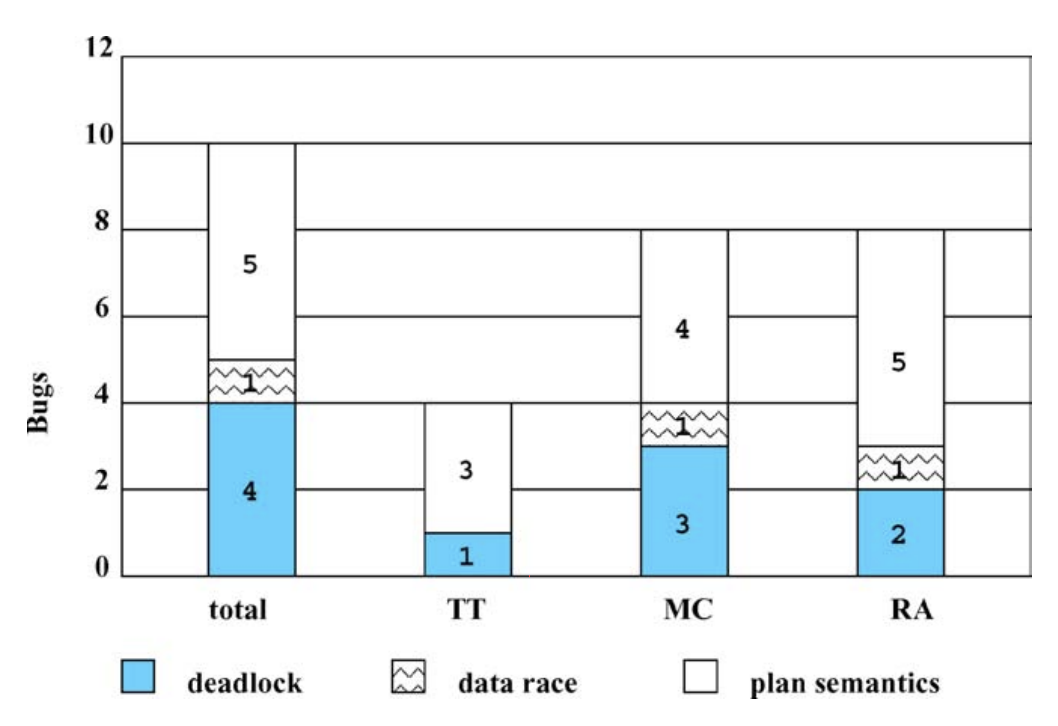
\includegraphics[scale=0.33]{fig2.png}
\caption{Desempe\~no de las diferentes t\'ecnicas} \label{fig2}
\end{figure}
La figura 2 muestra como se desempe\~naron las diferentes t\'ecnicas en la b\'usqueda de diez errores (4 deadlocks, 1 data race, 5 plan-related), los cuales a priori se conocia su existencia por el trabajo previo en el experimento. Las t\'ecnicas m\'as avanzadas como MC y RA resultaron ser m\'as eficientes en los errores relacionados a la concurrencia. El hecho de que TT haya sido peor que MC en todas las categorias fue un detalle un tanto inesperado.\\

\begin{figure}[H]
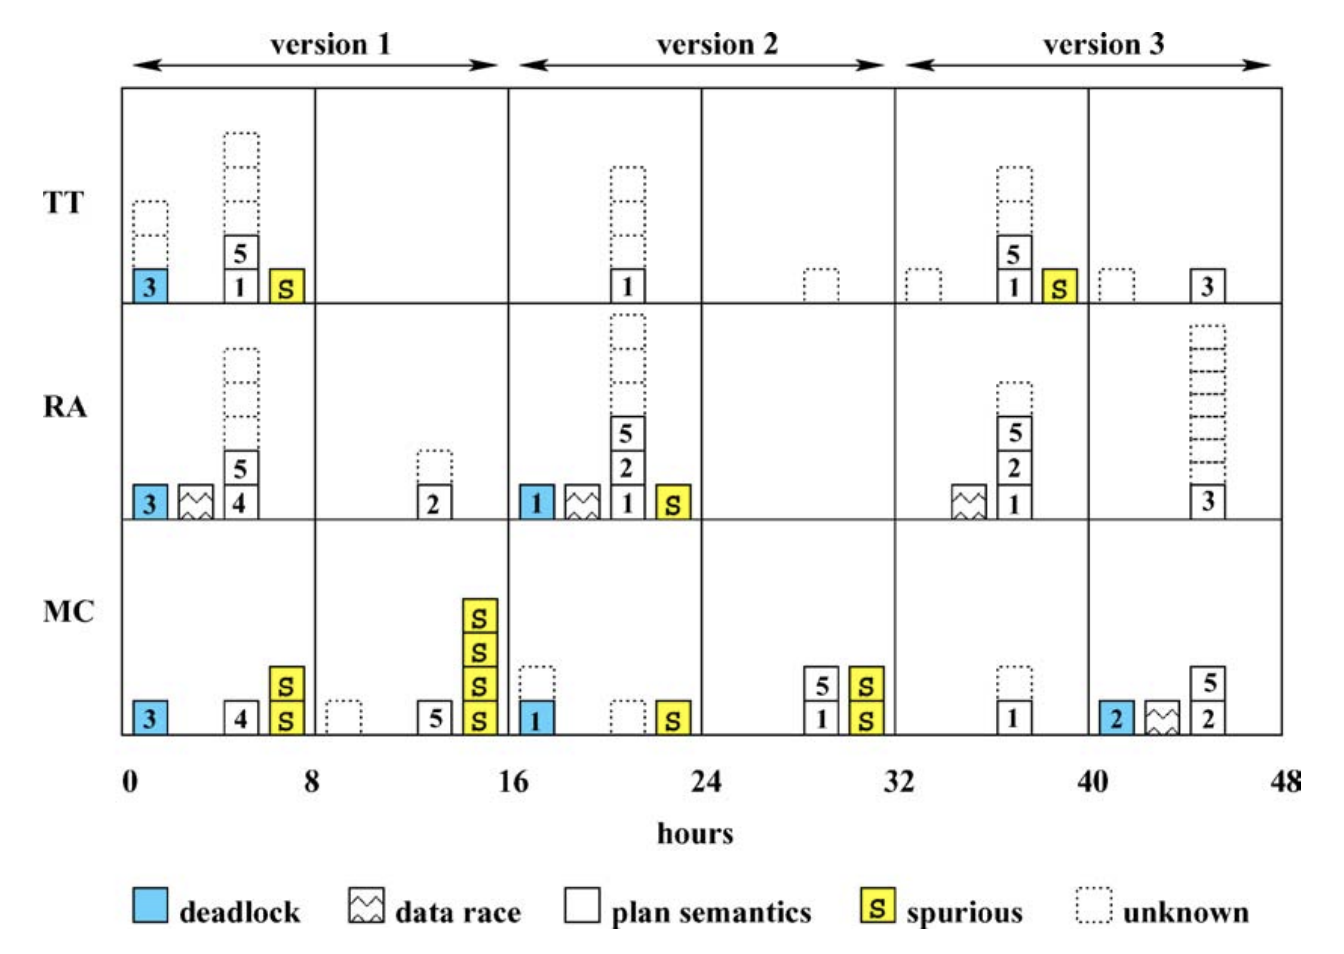
\includegraphics[scale=0.5]{fig3.png}
\caption{Errores encontrados a lo largo de las versiones} \label{fig3}
\end{figure}

En la figura 3 se puede observar el detalle por d\'ia de los bugs encontrados en una linea de tiempo de 48 horas (3 sesiones de 2 dias, cada dia consistiendo de 8 horas).\\ Una primera observaci\'on sobre MC, es que los Spurious Errors (errores introducidos a la hora de dise\~nar la abstracci\'on), decrementan a lo largo de las tres versiones de c\'odigo a verificar. Esto se debe a que los participantes se familiarizan con el c\'odigo y desarrollan mejores abstracciones. Deadlock 3 es simple y fue encontrado r\'apidamente por los tres m\'etodos. Deadlock 1 es un poco mas complejo pero fue encontrado por MC y RA, aunque TT nunca lo encontr\'o. Deadlock 2 fue el m\'as complejo y fue encontrado en la \'ultima versi\'on solo por MC. Respecto a los errores de Data Race, el equipo de MC solo intent\'o encontrar este tipo de errores al final del experimento, por eso s\'olo lo detect\'o en la \'ultima versi\'on. Un deadlock restante que ning\'un equipo encontr\'o, era extremadamente sutil y ven\'ia luego de un Data Race. A pesar de esto, se contaba con el error debido a que hab\'ia sido encontrado por JPF antes de comenzar el experimento.\\
Se midi\'o como los participantes dedicaron su tiempo en el an\'alisis a partir de cinco categorias:\\
\textbf{Delays}: incluye la espera de hardware y el tiempo en solucionar fallas en la tool, como tambi\'en el tiempo esperando un feedback.\\
\textbf{Setup/Preparation}: para el caso de MC incluy\'o el tiempo en crear las abstracciones, escribir las propiedades y test-cases.\\
\textbf{Running the Rover}: no fue muy relevante para MC pero si lo fue para RA y TT.\\
\textbf{Running the tool}: TT no utiliz\'o ninguna tool, pero MC y RA estuvieron basadas en tools.\\
\textbf{Result Analysis}: este es el tiempo destinado a determinar la causa del error. Para el caso de MC, esto significa determinar si el error es Spurious o no.\\
Enfoc\'andonos en los resultados obtenidos para model checker,  en la primer versi\'on de c\'odigo el equipo destino mayor cantidad de tiempo para la categor\'ia Delay y Setup/Preparation alrededor de 700 minutos el mismo tiempo que utilizaron ejecutando la herramienta.\\
En las siguientes dos versiones la distribuci\'on del uso del tiempo fue cambiando. En la \'ultima versi\'on de c\'odigo el equipo dedic\'o cerca de 1500 minutos exclusivamente a ejecutar la herramienta (m\'as del doble que en la primer versi\'on)
Durante la ejecuci\'on del JPF la mayor parte del tiempo fue invertido en probar diferentes estrategias de b\'usqueda para alcanzar las diferentes partes del espacio de estados. Eso se bas\'o en probar diferentes configuraciones de par\'ametros para el uso de heur\'isticas de b\'usquedas que provee la herramienta.\\
Esto da la pauta de que utilizar un Model Checker tal como lo es JPF requiere mas tiempo en crear un entorno ideal pero tiene mejor performance a la hora de encontrar errores.


\section{Comparaci\'on con otras herramientas}

JPF al trabajar con Java Bytecode, no requiere traducir ni armar otros modelos, algo que si se debe hacer en LTSA por ejemplo. En otras herramientas, es com\'un seleccionar propiedades (ya implementadas) que se quieran analizar, cosa que en JPF no sucede ya que se deben implementar (a no ser que se seleccione alguna que viene por defecto).
Otra diferencia a destacar, es que en LTSA se debe definir el algebra FSP de lo que se quiere modelar, mientras que JPF crea el modelo directamente a partir del codigo Java.
Cuando se utiliza JPF como model checker, es interesante obtener las trazas que llevan la ejecuci\'on a un estado de deadlock, para ello esta herramienta en caso de encontrar este tipo de trazas las muestra en el reporte de salida. De modo similar a lo que muestra LTSA.


\section{Conclusiones particulares}

JPF fue desarrollada con el objetivo de que sea una herramienta din\'amica y con la posibilidad de extenderla y/o adecuarla seg\'un el an\'alisis o estudio que se quiera realizar. La gran desventaja que tiene es que requiere grandes esfuerzos de configuraci\'on, ya que se deben setear propiedades, las cuales en muchos casos son dif\'iciles de entender e implementar y al momento de especificar software critico lo es m\'as a\'un, aunque en este caso, JPF es la soluci\'on ideal (No es casualidad que sea utilizado por la NASA). Pero todo esto genera que muchos usuarios no lo vean factible al uso de JPF.
No trabaja independientemente, ya que necesita de una terminal o IDEs, configuraciones y m\'odulos especificos para poder ejecutarlo y reportar resultados. Su instalaci\'on no es muy complicada, pero si puede serlo si no se cuenta de antemano con las herramientas que necesita JPF para poder ejecutarse. Al no contar con interfaz gr\'afica propia, se torna mas dif\'icil su uso, aunque lo positivo es que existen plugins que lo hacen menos complejo para usuarios que reci\'en comienzan a utilizar la terminal.\\
El constante desarrollo y creaci\'on de extensiones que se realiza en los principales eventos relacionados a la herramienta (Google Summer of Code[6], entre otros) permiten que la herramienta est\'e vigente todo el tiempo, amoldandos\'e a las necesidades de los usuarios.\\
Como conclusi\'on, m\'as all\'a de la complejidad de JPF en su todo, es una herramienta muy completa, que puede solucionar problemas sobre diversos campos de ejecuci\'on, de manera efectiva, seg\'un sus configuraciones y optimizaciones. Adem\'as, al ser una herramienta que trabaja puramente con java, lo hace m\'as \'util y popular a\'un.


%
% ---- Bibliography ----
%
% BibTeX users should specify bibliography style 'splncs04'.
% References will then be sorted and formatted in the correct style.
%
% \bibliographystyle{splncs04}
% \bibliography{mybibliography}
%

\begin{thebibliography}{8}
\bibitem{ref_url1}
Entrada Wikipedia Promela \url{https://en.wikipedia.org/wiki/Promela} \'Ultimo acceso 22 de Junio 2018

\bibitem{ref_url2}
P\'agina oficial Spin \url{http://spinroot.com/spin/whatispin.html} \'Ultimo acceso 22 de Junio 2018

\bibitem{ref_url3}
Brat, G., Drusinsky, D., Giannakopoulou, D. et al. Formal Methods in System Design (2004) 25: 167. https://doi.org/10.1023/B:FORM.0000040027.28662.a4

\bibitem{ref_url4}
P. C. Mehlitz, "Trust Your Model - Verifying Aerospace System Models with Java Pathfinder," 2008 IEEE Aerospace Conference, Big Sky, MT, 2008, pp. 1-11.
doi: 10.1109/AERO.2008.4526573

\bibitem{ref_url5}
Fujitsu - \url{http://www.fujitsu.com/global/about/resources/news/press-releases/2010/0112-02.html} \'Ultimo acceso 22 de Junio 2018

\bibitem{ref_url6}
Google Summer of Code - \url{https://summerofcode.withgoogle.com/?csw=1} \'Ultimo acceso 22 de Junio 2018

\bibitem{ref_url7}
Java PathFinder for Android Devices - \url{https://bitbucket.org/matsurago/jpf-mobile-devices/wiki/Home} \'Ultimo acceso 22 de Junio 2018

\bibitem{ref_url8}
M. Milewicz, Reed and Poulding, Simon. (2018). Scalable Parallel Model Checking via Monte-Carlo Tree Search. ACM SIGSOFT Software Engineering Notes. 42. 1-5. 10.1145/3149485.3149495. 


\bibitem{ref_url9}
Search Component \url{https://github.com/javapathfinder/jpf-core/wiki/Search-Strategies} \'Ultimo acceso 22 de Junio 2018

\bibitem{ref_url10}
Entrada Wikipedia B\'usqueda en profundidad \url{https://en.wikipedia.org/wiki/Depth-first\_search} \'Ultimo acceso 22 de Junio 2018

\bibitem{ref_url11}
Entrada Wikipedia Partial Order Reduction \url{http://en.wikipedia.org/wiki/Partial\_order\_reduction} \'Ultimo acceso 22 de Junio 2018

\end{thebibliography}
\end{document}
